% !TEX root = ../../../main.tex
% 来源：中学数学实验教材·第三册（高中数学）
% 章节：函数及其图象 / 一次函数（线性函数）
% 原始文件：4.tex，行 2351-2367
% 类型：tikz
% ---
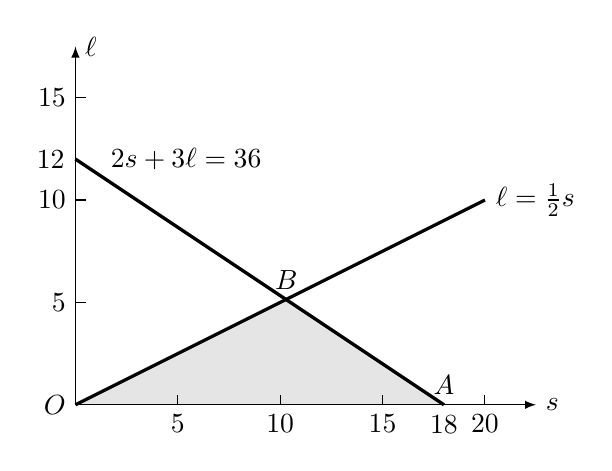
\begin{tikzpicture}[>=latex, scale=1.3]
\fill[gray!20] (0,0)--(2.06,1.03)--(3.6,0)--(0,0);

    \draw[->] (0,0) --(4.5,0)node[right]{$s$};
    \draw[->] (0,0)node[left]{$O$}--(0,3.5)node[right]{$\ell$};
\foreach \x in {5,10,15}
{
    \draw(\x/5,0)node[below]{$\x$}--(\x/5,.1);
    \draw(0,\x/5)node[left]{$\x$}--(.1,\x/5);
}
\draw(4,0)node[below]{20}--(4,.1);
\node at (0.25,2.4)[right]{$2s+3\ell=36$};
\draw[very thick](0,2.4)node[left]{12}--(3.6,0)node[below]{18};
\node at (3.6,0)[above]{$A$};
\draw[very thick] (0,0)--(4,2)node[right]{$\ell=\frac{1}{2}s$};
\node at (2.06,1.03)[above]{$B$};
\end{tikzpicture}
